\documentclass[aspectratio=169]{beamer}
\usepackage[T1]{fontenc}
\usepackage[utf8]{inputenc}
\usepackage{lmodern}
\usepackage{microtype}
\usepackage{xcolor}
\usepackage{tikz}
\usetikzlibrary{positioning, arrows.meta, calc}
\usepackage{fontawesome5}
\definecolor{wurgreen}{HTML}{34B233}
\definecolor{darkgreen}{HTML}{1F6B1E}
\definecolor{darknavy}{HTML}{1A1A2E}
\definecolor{midgray}{HTML}{6B7280}
\definecolor{lightgray}{HTML}{F3F4F6}
\definecolor{lightgreen}{HTML}{E8F7E8}
\definecolor{bodytext}{HTML}{1F2937}
\definecolor{warnred}{HTML}{FEE2E2}
\definecolor{warnborder}{HTML}{EF4444}
\definecolor{codebg}{HTML}{1E1E2E}
\definecolor{codegreen}{HTML}{9ECE6A}
\definecolor{codeblue}{HTML}{7AA2F7}
\definecolor{codeorange}{HTML}{FF9E64}
\definecolor{codegray}{HTML}{C0CAF5}
\usetheme{default}\usecolortheme{default}\usefonttheme{professionalfonts}
\setbeamertemplate{navigation symbols}{}
\setbeamertemplate{itemize items}{\textcolor{wurgreen}{\textbullet}}
\setbeamertemplate{itemize subitem}{\textcolor{midgray}{--}}
\setbeamercolor{frametitle}{fg=white, bg=darknavy}
\setbeamerfont{frametitle}{size=\large, series=\bfseries}
\setbeamertemplate{frametitle}{%
  \begin{beamercolorbox}[wd=\paperwidth, ht=1.1cm, dp=0.2cm, leftskip=0.6cm]{frametitle}
    \usebeamerfont{frametitle}\insertframetitle\end{beamercolorbox}}
\setbeamercolor{background canvas}{bg=white}
\setbeamercolor{normal text}{fg=bodytext}
\setbeamertemplate{footline}{%
  \begin{beamercolorbox}[wd=\paperwidth, ht=0.4cm, dp=0.15cm]{footline}
    \hspace{0.5cm}\textcolor{midgray}{\tiny Introduction to Python · Module 5: Strings \& Files}%
    \hfill\textcolor{midgray}{\tiny \insertframenumber}\hspace{0.4cm}\end{beamercolorbox}}
\newcommand{\codebox}[1]{\begin{center}
  \begin{tikzpicture}\node[fill=codebg, rounded corners=4pt, inner sep=9pt, text width=0.85\textwidth, text=codegray]{\ttfamily\small #1};\end{tikzpicture}\end{center}}
\begin{document}
{\setbeamertemplate{footline}{}
\begin{frame}[plain]
  \begin{tikzpicture}[remember picture, overlay]
    \fill[darknavy] (current page.south west) rectangle (current page.north east);
    \fill[wurgreen] (current page.south west) rectangle ([xshift=0.45cm]current page.north west);
    \node[anchor=west, text=white, font=\huge\bfseries, text width=13cm] at ([xshift=1.1cm, yshift=1.4cm]current page.west){Introduction to Python};
    \node[anchor=west, text=wurgreen, font=\large, text width=12cm] at ([xshift=1.1cm, yshift=0.2cm]current page.west){Module 5 --- Strings \& Files};
    \node[anchor=west, text=midgray, font=\small, text width=12cm] at ([xshift=1.1cm, yshift=-1.3cm]current page.west){String methods, splitting, and file I/O};
  \end{tikzpicture}
\end{frame}}

\begin{frame}{Strings Are Powerful}
\vspace{0.2cm}
{\small Text is central to a lot of research, and Python strings come with dozens of useful
\textbf{methods}. A method is a function attached to a value, called with a dot.}
\medskip
\codebox{%
text \textcolor{codegray}{=} \textcolor{codegreen}{"  Hello World  "}\\[6pt]
text.\textcolor{codeblue}{lower}()\quad\ \ \ \ \textcolor{codegray}{\# "  hello world  "}\\
text.\textcolor{codeblue}{upper}()\quad\ \ \ \ \textcolor{codegray}{\# "  HELLO WORLD  "}\\
text.\textcolor{codeblue}{strip}()\quad\ \ \ \ \textcolor{codegray}{\# "Hello World" (trim spaces)}\\
text.\textcolor{codeblue}{replace}(\textcolor{codegreen}{"World"}, \textcolor{codegreen}{"Python"})}
\medskip
{\small\textcolor{midgray}{\textit{These are exactly the operations behind text
preprocessing --- lowercasing, trimming, cleaning.}}}
\end{frame}

\begin{frame}{Splitting \& Joining}
\vspace{0.2cm}
{\small Two workhorse methods for turning text into lists and back --- the heart of
tokenization.}
\medskip
\codebox{%
sentence \textcolor{codegray}{=} \textcolor{codegreen}{"the cat sat"}\\[6pt]
\textcolor{codegray}{\# split a string into a list of words}\\
words \textcolor{codegray}{=} sentence.\textcolor{codeblue}{split}()\quad\textcolor{codegray}{\# ["the", "cat", "sat"]}\\[6pt]
\textcolor{codegray}{\# join a list back into a string}\\
\textcolor{codegreen}{" "}.\textcolor{codeblue}{join}(words)\quad\ \ \ \ \ \ \textcolor{codegray}{\# "the cat sat"}\\
\textcolor{codegreen}{"-"}.\textcolor{codeblue}{join}(words)\quad\ \ \ \ \ \ \textcolor{codegray}{\# "the-cat-sat"}}
\medskip
{\small \texttt{split()} on nothing splits on spaces; \texttt{split(",")} splits on commas
(handy for CSV lines). \texttt{join()} glues a list together with the string you call it on.}
\end{frame}

\begin{frame}{Checking \& Finding in Strings}
\vspace{0.2cm}
\codebox{%
word \textcolor{codegray}{=} \textcolor{codegreen}{"policy"}\\[6pt]
\textcolor{codegreen}{"pol"} \textcolor{codeblue}{in} word\quad\ \ \ \ \ \textcolor{codegray}{\# True  (substring check)}\\
word.\textcolor{codeblue}{startswith}(\textcolor{codegreen}{"pol"})\quad\textcolor{codegray}{\# True}\\
word.\textcolor{codeblue}{endswith}(\textcolor{codegreen}{"cy"})\quad\ \ \textcolor{codegray}{\# True}\\
word.\textcolor{codeblue}{count}(\textcolor{codegreen}{"o"})\quad\ \ \ \ \ \ \textcolor{codegray}{\# 1}\\
\textcolor{codeblue}{len}(word)\quad\ \ \ \ \ \ \ \ \ \ \ \textcolor{codegray}{\# 6}}
\medskip
{\small The \texttt{in} keyword works on strings (``is this substring present?'') just like it
works on lists. These checks are the building blocks of filtering and searching text.}
\end{frame}

\begin{frame}{Reading \& Writing Files}
\vspace{0.2cm}
{\small Real data lives in files. The safe way to open one is with a \texttt{with} block --- it
closes the file automatically when you're done.}
\medskip
\codebox{%
\textcolor{codegray}{\# writing}\\
\textcolor{codeblue}{with} \textcolor{codeblue}{open}(\textcolor{codegreen}{"notes.txt"}, \textcolor{codegreen}{"w"}) \textcolor{codeblue}{as} f:\\
\quad f.\textcolor{codeblue}{write}(\textcolor{codegreen}{"Hello file"})\\[6pt]
\textcolor{codegray}{\# reading}\\
\textcolor{codeblue}{with} \textcolor{codeblue}{open}(\textcolor{codegreen}{"notes.txt"}) \textcolor{codeblue}{as} f:\\
\quad content \textcolor{codegray}{=} f.\textcolor{codeblue}{read}()}
\medskip
{\small The mode \texttt{"w"} \textbf{writes} (overwrites!), \texttt{"r"} \textbf{reads} (the
default), \texttt{"a"} \textbf{appends}. For structured data (CSVs, spreadsheets), you'll use
\textbf{pandas} --- coming next.}
\end{frame}

\begin{frame}{Module 5: Takeaways}
\vspace{0.3cm}
\begin{itemize}\setlength\itemsep{8pt}
  \item[\textcolor{wurgreen}{\faCheck}] String \textbf{methods}: \texttt{.lower() .upper() .strip() .replace()}
  \item[\textcolor{wurgreen}{\faCheck}] \texttt{.split()} makes a list of words; \texttt{.join()} glues them back
  \item[\textcolor{wurgreen}{\faCheck}] \texttt{in}, \texttt{.startswith()}, \texttt{.count()} check and search text
  \item[\textcolor{wurgreen}{\faCheck}] Open files safely with \texttt{with open(...) as f:}
  \item[\textcolor{wurgreen}{\faCheck}] Modes: \texttt{"r"} read, \texttt{"w"} write, \texttt{"a"} append
\end{itemize}
\medskip
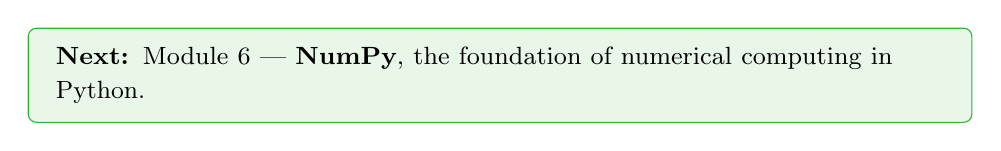
\begin{tikzpicture}
  \node[fill=lightgreen, draw=wurgreen, rounded corners=3pt, inner xsep=10pt, inner ysep=7pt, text width=\textwidth-24pt]{%
    {\small \textbf{Next:} Module 6 --- \textbf{NumPy}, the foundation of numerical computing in
    Python.}};
\end{tikzpicture}
\end{frame}
\end{document}
